\documentclass[a4paper,12pt]{article}


\usepackage{relsize}
\usepackage[margin=3cm]{geometry} %Definiere Rand
\usepackage{graphicx} % Zum Einbinden von Bildern
\usepackage[english]{babel} % Direkte Eingabe von Umlauten
%\usepackage[utf8]{inputenc} % Direkte Eingabe von Umlauten
\UseRawInputEncoding
\usepackage[T1]{fontenc}  % Direkte Eingabe von Umlauten
\usepackage{pgfplots} % Zum Einfuegen von Plots
\pgfplotsset{compat=1.14} % Damit wird beim Plotten keinen Error bekommen
\usepackage[section]{placeins} %Damit Bilder in der Section bleiben
\usepackage{amsmath} % Standard fuer mathematische Ausdruecke
\usepackage{amssymb} % Weitere Symbole
\usepackage{mathtools} % Fuer weitere mathematische Ausdruecke
\usepackage{siunitx} % Um SI-Einheiten anzugeben
\usepackage[font=small,labelfont=bf]{caption} % Kleinerer Text bei Captions
\usepackage{tabu} % Anderes Tabellenenvironment, wird am Ende fuer die Namen verwendet
\usepackage{subcaption} % Side-by-side figures with minipage
\usepackage{url} % Damit man urls zitieren kann
\usepackage[autostyle=true,german=quotes]{csquotes} % Damit Zitieren leichter ist; Bsp: \enquote{nur}
\usepackage[nottoc,numbib]{tocbibind} % Damit die Referenzen im Inhaltsverzeichnis erscheinen
% Die folgenden zwei Zeilen benennen "Inhaltsverzeichnis" zu "Referenzen um
\usepackage{standalone} % Zum Outsourcen von Plots
\addto\captionsngerman{\renewcommand{\bibname}{Referenzen} \renewcommand{\refname}{Referenzen}} % Benennt "Literatur" in "Referenzen" um
\sisetup{range-phrase=-} % Wie SI-Intervalle angezeigt werden
\usepackage{setspace} % Damit die naechsten funktionieren
\renewcommand{\topfraction}{0.85} % Let top 85% of a page contain a figure
\renewcommand{\textfraction}{0.1} % Default amount of minimum text on page (Set to 10%)
\renewcommand{\floatpagefraction}{0.75} % Only place figures by themselves if they take up more than 75% of the page
\DeclareSIPostPower\tothefourth{4} % SI-Einheiten zur 4. Potenz
%
\makeatletter
\newcommand*{\rom}[1]{\expandafter\@slowromancap\romannumeral #1@}
\makeatother %roman numerals
\usepackage{threeparttable, tablefootnote}
\DeclareSIUnit\torr{torr}
\usepackage{circuitikz} %For circuits
\renewcommand{\d}{\mathrm{d}}
\newcommand{\intl}{\int\limits}
\sisetup{math-micro=\text{µ},text-micro=µ}
\usepackage{hyperref} % For hyperlinks to be clickable

\usepackage{listings} % For embedding code into the document
\usepackage{jlcode} % Add julia syntax to listings package
\lstset{language=Julia}

\begin{document}
%
    \title{Cavity QED with cold particles\\
    \vspace{2em}
    Bachelorarbeit\\
    \vspace{2em}
    \smaller[2]{}zur Erlangung des akademischen Grades\\
    Bachelor of Science (BSc)\\
    \vspace{2em}
    eingereicht an der\\
    Fakult{\"a}t f{\"u}r Mathematik, Informatik und Physik\\
    der\\
    Leopold-Franzens-Universit{\"a}t Innsbruck\\
    \vspace{1.5em}
    von}

    \author{
 	\LARGE Bernhard Gstrein\\
 	\vspace{.5em} \\
 	Betreuer:\\
 	Univ.Prof. Dr. Helmut Ritsch\\
 	\small Institut f{\"u}r Theoretische Physik\\
 	\vspace{1em}
	}
    
\date{Innsbruck, 2019}

\maketitle
   
\begin{abstract}
\noindent We motivate and derive a theoretical model arranging atoms in a lattice to simulate a solid. For that, we'll make use of atom-light field interaction which is enhanced in a cavity. After deriving the Hamiltonians for our systems, we'll discuss some of their properties. We'll then conduct simulations in the language Julia with the framework QuantumOptics.jl to see if we can observe the properties we expect our systems to have.
\end{abstract}
   
\newpage
   
\tableofcontents
 
\newpage
    

\section{Introduction}
The study of solid-state objects is of great interest for us, especially since some phenomena occuring in solids have a lot of commercial potential. There are some difficulties, however. It can be very challenging to look into a solid. Certain phenomena might be happening very fast (e.g. on a nanosecond scale), the lattice spacing might be very small (e.g. only several angstroms apart) and in every naturally occuring solid there are structural defects and lattice vibrations. All these things can obfuscate the basic workings of certain phenomena. On top of all that, we can't change a naturally occuring solid which is probably the biggest inconvenience. A way to circumvent all these problems is to just make a crystal ourselves, a crystal in which certain phenomena are happening much slower (e.g. on a second scale), in which there's a bigger lattice spacing (e.g. on a micrometer scale) and that is free of defects. That crystal will be fully controllable by us and we can change its structure as we wish.

In this thesis, we'll ask ourselves the question how to make atoms self-organize to create an artificial solid. For that, we'll establish a theoretical model in which we arrange atoms in a lattice. We'll obtain two configurations with two Hamiltonians whose properties we'll discuss. Simulations in the language Julia with the framework QuantumOptics.jl will show us if we're able to observe the properties that we expect.

\section{Explanation of the model}

What we want to achieve is to arrange atoms in a lattice to simulate a solid. We need to somehow hold them in place. For that, we'll use laser light. Consider the setup depicted in Figure~\ref{counter-propagating}. There are two lasers, each with the same frequency. If we set their direction on the same axis, but counter propagating with contributions $\propto \exp(ikx)$ and $\propto \exp(-ikx)$, a cosine pattern or standing wave of the intensity will form. In between, we put our atoms. There's a special trick now. We set the frequency of the laser $\omega_\text{l}$ way below the excitation frequency of the atoms $\omega_\text{a}$ (this is commonly called "red-detuning"). That will induce dipoles in the atoms and the dipoles will interact with the light field. Because of the dipole-light field interaction, there's now a potential for the atoms which is what we needed. The atoms will now sort of "fall" into the lowest points of the potential to minimize their energy. The light field intensity has a cosine pattern, thus the same will be the case for the potential ($V \propto -I$). Now we have an array of equally spaced atoms, already what we could call an artificial solid. To enhance atom-light field interaction, we'll take our setup one step further and introduce a cavity, as depicted in Figure~\ref{put_in_cavity}. There are two mirrors. The one on the left is partially transmissive to let the laser light in. We set the distance between the two mirros to $d = n \lambda / 2$ so that the light field will be amplified inside the cavity.

\begin{figure}[!htb]
	\begin{minipage}[b]{.5\linewidth}
	\centering
	\includegraphics[width=.7\linewidth]{images/counter_propagating.eps}
	\subcaption{Counter-propagating lasers.}
	\label{counter-propagating}
	\end{minipage}
%
	\begin{minipage}[b]{.5\linewidth}
	\centering
	\includegraphics[width=.7\linewidth]{images/cavity.eps}
	\subcaption{Optical cavity.}
	\label{put_in_cavity}
	\end{minipage}
\caption{Two counter-propagating lasers create a cosine-potential. In between, we put our atoms. Red-detuning the lasers will induce dipoles in the atoms which interact with the light field, creating a potential for the atoms. As the atoms always strive to minimize their energy, they will position themselves at the "valleys" of the potential. We'll take that approach even further and put the atoms in a cavity. That way atom-light field interaction will be enhanced.}
\label{laser_cavity}
\end{figure}
\FloatBarrier

\noindent There are different ways to get a light field inside the cavity. Figure~\ref{longitudinal_pump} depicts what we've discussed so far. There we shoot a laser parallel to the cavity axis into the cavity (longitudinal pump). Even if there are no atoms inside, there's still a light field. That is not the case if we pump transverally, as described in \cite{domokos2002} and shown in Figure~\ref{transversal_pump}. For transversal pump, if there are no atoms inside the cavity, no light field will exist along the cavity axis. To create a light field, here we rely on the atoms scattering the photons into the cavity, i.e. the atoms effectively create their own trapping potential. Pumping transversally, a couple interesting phenomena emerge which do not happen for the longitudinal pump. We will discuss those properties later. Now to the derivation of the Hamiltonians for those two systems.

\begin{figure}[!htb]
	\begin{minipage}[b]{.5\linewidth}
	\centering
	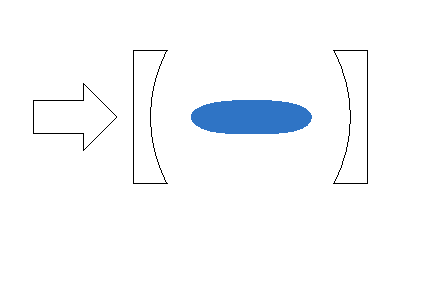
\includegraphics[width=.8\linewidth]{images/pump_long.eps}
	\subcaption{Longitudinal pumping.}
	\label{longitudinal_pump}
	\end{minipage}
%
	\begin{minipage}[b]{.5\linewidth}
	\centering
	\includegraphics[width=.8\linewidth]{images/pump_trans.eps}
	\subcaption{Transversal pumping.}
	\label{transversal_pump}
	\end{minipage}
\caption{Longitudinally and transversally pumped cavities. For longitudinal pumping, even if there are no atoms inside the cavity, there's still a light field. That is not the case for transversal pumping. There the light field along the cavity axis is created by the atoms scattering incoming photons, i.e. the atoms are effectively creating their own trapping potential.}
\label{pumping}
\end{figure}
\FloatBarrier

\section{Derivation of the Hamiltonians}
For those wishing to refresh their knowledge in quantum mechanics, the introductory chapters of Fox's quantum optics book will be of great help \cite{fox} (it's a great quantum optics book in general). In this section we'll derive the Hamiltonians being used for the simulation: One Hamiltonian for longitudinal pumping and one for transversal pumping. We'll start with the Jaynes-Cummings Hamiltonian which describes the interaction of a two-level atom with a single mode of a cavity-field. We'll then modify the Hamiltonian according to our needs step by step. We'll tackle the crucial details and reference parts of the derivation which are not presented here.

\subsection{The Jaynes-Cummings Hamiltonian}
The Jaynes-Cummings model describes the interaction of a two-level atom with a single mode of a cavity field. The first appearance of the model was in \cite{jaynes}. Since we're dealing with both an atom and a light field at the same time, we have a composite system, i.e.

\begin{align}
\psi_\text{total} = \psi_\text{light} \otimes \psi_\text{atom}.
\end{align}The fact that we have two levels motivates a two-dimensional basis for the atom:

\begin{align}
|\text{g}\rangle = \begin{pmatrix}0 \\ 1\end{pmatrix}, && |\text{e}\rangle = \begin{pmatrix}1 \\ 0\end{pmatrix},
\end{align}where $|\text{g}\rangle$ is the ground state and $|\text{e}\rangle$ is the excited state. Both states respond to the operators

\begin{align}
\sigma^+ = \begin{pmatrix}0 & 1 \\ 0 & 0\end{pmatrix}, && \sigma^- = \begin{pmatrix}0 & 0 \\ 1 & 0\end{pmatrix},
\end{align}where $\sigma^+$ is the raising operator and $\sigma^-$ is the lowering operator. They have the properties

\begin{align}
\sigma^+ |\text{g}\rangle = |\text{e}\rangle, && \sigma^- |\text{e}\rangle = |\text{g}\rangle.
\end{align}The wave function for the atoms depends on the position, while this is not the case for the light field. Instead we will use photon number states or Fock states. A photon number state $|n\rangle$ thus represents a monochromatic quantized field containing $n$ atoms. The ground state $|0\rangle$ corresponds to 0 photons. The creation and  annihilation operators $a^\dagger$ and $a$ correspond to creating and annihilating a photon. We'll restrict ourselves to one dimension and start with an atom (or a Bose-Einstein condensate) in an external potential:

\begin{align}
H_0 = \frac{p^2}{2m} + V_\text{ext}(x).
\end{align}Now we place that atom in a cavity and it will interact with the cavity mode, creating more terms in our Hamiltonian that we have to consider. First, there's the energy of the field:

\begin{align}
H_\text{field} = -\hbar \omega_\text{c} a^\dagger a,
\end{align}where $\omega_\text{c}$ is the resonance frequency of the cavity and $a^\dagger$ and $a$ are the creation and annihilation operators. Next, we'll add a term describing the atomic transitions:

\begin{align}
H_\text{transition} = -\hbar \omega_\text{a} \sigma_z,
\end{align}where $\omega_\text{a}$ is the resonance frequency of the atom and $\sigma_z$ is the Pauli $z$-matrix which is defined as $\sigma_z = 1/2(|\text{e}\rangle \langle \text{e}| + |\text{g} \rangle \langle \text{g}|)$ or

\begin{align}
\sigma_z = \begin{pmatrix}1/2 & 0 \\ 0 & -1/2\end{pmatrix}.
\end{align} The Hamiltonian $H_\text{transition}$ describes the atom being in the ground state or excited state, the transition energy is $\hbar \omega_\text{a}$. The atom-field interaction we describe with following term:

\begin{align}
H_\text{interaction} = \hbar g_0 \cos(kx) (\sigma^+ a + \sigma^- a^\dagger),
\end{align}where $g_0$ is the coupling strength. Finally, we'll add the term describing the pumping:

\begin{align}
H_\text{pump} = \hbar \eta (a e^{i\omega_\text{l}t} + a^\dagger e^{-i\omega_\text{l}t}),
\end{align}where $\eta$ is the pumping strength and $\omega_\text{l}$ is the laser frequency. We now have the full Jaynes-Cummings Hamiltonian which is the sum of all terms above:

\begin{align}
\begin{split}
H_\text{JC} = \underbrace{p^2 / 2m}_\text{atom} + \underbrace{V_\text{ext}(x)}_\text{external potential} - \underbrace{\hbar \omega_\text{a} \sigma_z}_\text{atomic transitions} - \underbrace{\hbar \omega_\text{c} a^\dagger a}_\text{field} + \underbrace{\hbar \eta (a e^{i \omega_\text{l} t} + a^\dagger e^{-i \omega_\text{l} t})}_\text{pumping} + \\
+ \underbrace{\hbar g_0 \cos(kx) (\sigma^+ a + \sigma^- a^\dagger)}_\text{field-atom interaction}.
\end{split}
\end{align}A more detailed derivation of the Jaynes-Cummings Hamiltonian (starting from Maxwell's equations and quantizing the cavity mode) can be found at \cite{collapseandrevival}. In order to get rid of the explicit time-dependence, we transform the Hamiltonian to a frame rotating with $\omega_\text{l}$. The Hamiltonian now reads:

\begin{align}
\begin{split}
H_\text{JC} = \frac{p^2}{2m} + V_\text{ext}(x) + \hbar \Delta_\text{a} \sigma_z - \hbar \Delta_\text{c} a^\dagger a + \hbar \eta (a + a^\dagger) + \\
+ \hbar g_0 \cos(kx) (\sigma^+ a + \sigma^- a^\dagger),
\end{split}
\end{align}where $\Delta_\text{a} = \omega_\text{l} - \omega_\text{a}$ and $\Delta_\text{c} = \omega_\text{l} - \omega_\text{c}$.

\subsection{Detuning}
The derivation for the Hamiltonians for the following sections is taken from \cite{donner}. Now we derive heuristically a modified Hamiltonian. Going to the Heisenberg picture, we get:

\begin{align}
\dot{a} = \frac{i}{\hbar} [H, a] = i \Delta_\text{c} a - i \eta -i g_0 \cos(kx) \sigma^-.
\label{a_dot}
\end{align}Obviously, the kinetic energy and potential term vanish under the commutator. For the other terms:

\begin{align}
a^\dagger a = N, \qquad [N, a] = -a, \\
(a + a^\dagger) a - a (a + a^\dagger) = aa + a^\dagger a - aa - aa^\dagger & = 1 \\
\text{because we know:} \quad aa^\dagger & = a^\dagger a + 1, \nonumber \\
[\sigma^+ a + \sigma^- a^\dagger, a] = \sigma^+ \underbrace{[a, a]}_{0} + \sigma^- \underbrace{[a^\dagger, a]}_{1} = \sigma^-.
\end{align}The creation and annihilation operators ($a^\dagger$ and $a$) and the raising and lowering operators ($\sigma^+$ and $\sigma^-$) live in different Hilbert spaces and thus don't influence each other. A good reference for the commutator relation is \cite{bertlmann}. The time-derivative for the raising operator reads:

\begin{align}
\dot{\sigma}^+ = \frac{i}{\hbar} [H, \sigma^+] = \underbrace{-i \Delta_\text{a} \sigma^+}_{(*)} + \underbrace{i g_0 \cos(kx) a^\dagger}_{(**)}.
\end{align}For ($\ast$), we'll look at the matrix representation of the operators:

\begin{align}
\sigma^+ = \begin{pmatrix}0 & 1 \\ 0 & 0\end{pmatrix}, \quad \sigma^- = \begin{pmatrix}0 & 0 \\ 1 & 0\end{pmatrix}, \quad \sigma_z = \begin{pmatrix}1/2 & 0 \\ 0 & -1/2\end{pmatrix}.
\end{align}We calculate the commutator relation $[\sigma_z, \sigma^+]$ explicitly:

\begin{align}
[\sigma_z, \sigma^+] & = \begin{pmatrix}1/2 & 0 \\ 0 & -1/2\end{pmatrix} \begin{pmatrix}0 & 1 \\ 0 & 0\end{pmatrix} - \begin{pmatrix}0 & 1 \\ 0 & 0\end{pmatrix} \begin{pmatrix}1/2 & 0 \\ 0 & -1/2\end{pmatrix} = \nonumber \\[5pt]
& = \begin{pmatrix}0 & 1/2 \\ 0 & 0\end{pmatrix} - \begin{pmatrix}0 & -1/2 \\ 0 & 0\end{pmatrix} = \begin{pmatrix}0 & 1 \\ 0 & 0\end{pmatrix} = \sigma^+.
\end{align}For ($\ast \ast$), we'll calculate $[\sigma^-, \sigma^+]$:

\begin{align}
[\sigma^-, \sigma^+] & = \begin{pmatrix}0 & 0 \\ 1 & 0\end{pmatrix} \begin{pmatrix}0 & 1 \\ 0 & 0\end{pmatrix} - \begin{pmatrix}0 & 1 \\ 0 & 0\end{pmatrix} \begin{pmatrix}0 & 0 \\ 1 & 0\end{pmatrix} = \nonumber \\[5pt]
& = \begin{pmatrix}0 & 0 \\ 0 & 1\end{pmatrix} - \begin{pmatrix}1 & 0 \\ 0 & 0\end{pmatrix} = \begin{pmatrix}-1 & 0 \\ 0 & 1\end{pmatrix} = -2\sigma_z \approx 1.
\end{align}In our case, the pumping laser is far detuned from the atomic resonance frequency, i.e. $\omega_\text{l} \ll \omega_\text{a}$. The atom thus only stays in the ground state and we approximate $\sigma_z \approx -1/2$. Since we're not interested in fast dynamics, we set $\dot{\sigma}^+ = 0$. We get:

\begin{align}
\sigma^+ = \frac{g_0 }{\Delta_\text{a}} \cos(kx) a^\dagger, && \sigma^- = \frac{g_0 }{\Delta_\text{a}} \cos(kx) a.
\end{align}Putting the above relation in equation~\ref{a_dot}, we get:

\begin{align}
\dot{a} = -i \Delta_\text{c} a + \frac{i g_0}{\Delta_\text{a}}  \cos(kx) a - i \eta.
\end{align}We can thus make a guess of the effective Hamiltonian:

\begin{align}
H_\text{long} = \frac{p^2}{2m} + V_\text{ext}(x) - \hbar \Delta_\text{c} a^\dagger a + \hbar \eta (a + a^\dagger) + \hbar U_0 \cos(kx)^2 a^\dagger a,
\end{align}where we set $U_0 \coloneqq g_0^2 / \Delta_\text{a}$. Note that because $H_\text{long} \propto \cos(kx)^2$, the Hamiltonian is $\lambda / 2$-periodic. Later in the simulation program, we want to make sure all quantities are expressed in terms of the recoil energy $E_r = \hbar \omega_r$, where $\omega_r = \hbar k^2 / 2m$ is the recoil frequency. Therefore we factor our $E_r$ to see what we have to type into the program:

\begin{align}
\begin{split}
H_\text{long} = \hbar \omega_r \biggl( \frac{1}{\hbar^2 k^2} p^2 + \frac{1}{\hbar \omega_r} V_\text{ext}(x) - \frac{1}{\omega_r} \Delta_c a^\dagger a + \frac{1}{\omega_r} \eta (a + a^\dagger) + \\
 + \frac{1}{\hbar \omega_r} U_0 \cos(kx)^2 a^\dagger a \biggr).
\end{split}
\end{align}In the simulation program, we will set $\hbar = 1$ and multiply each quantity by the preceding factors.

\subsection{Transversal Pump}

Now we'll tackle the transversal pump. Here the cavity mode will only be populated by photons which were scattered off the atoms. The Hamiltonian now reads:

\begin{align}
\begin{split}
H_\text{trans} = \frac{p^2}{2m} + V_\text{ext}(x) - \hbar \Delta_\text{c} a^\dagger a  + \hbar \eta \cos(kx) \cos(kz) (a + a^\dagger) + \\
+ \hbar \frac{\Omega^2}{\Delta_\text{a}} \cos(kz)^2 + \hbar U_0 \cos(kx)^2 a^\dagger a,
\end{split}
\end{align}where $\Omega$ is the Rabi frequency. Here we only consider one dimension, so we set $z=0$:

\begin{align}
\begin{split}
H_\text{transv} = \frac{p^2}{2m} + V_\text{ext}(x) - \hbar \Delta_c a^\dagger a + \hbar \eta \cos(kx) (a + a^\dagger) + \\
 + \hbar U_0 \cos(kx)^2 a^\dagger a.
\end{split}
\end{align}Note that because $H_\text{trans} \propto \cos(kx)$, the Hamiltonian is $\lambda$-periodic. The only difference now to the longitudinal pump Hamiltonian is the spatial dependence in the pump term.

\section{Properties of the system}

\noindent We'll now discuss some properties that the longitudinally and transversally pumped cavities have and later tackle some further details only concerning the transversally pumped cavity. There is a fundamental difference how atoms scatter light in the longitudinally pumped cavity and in the transversally pumped cavity. For the longitudinal pump, if a photon with momentum $\hbar k$ in $x$-direction bumps into an atom, it will recoil backward, having now a momentum $-\hbar k$. Conservation of momentum thus requires the atom to have now a momentum of $2\hbar k$. For the transversal pump, when a photon is incident perpendicularly to the cavity axis, the total momentum in the $x$-direction will be 0. If an atom scatters now the photon along the cavity axis, it will now have a momentum of $\hbar k$ and the photon $-\hbar k$. The total momentum along the $x$-direction will still be 0. We see that the fundamental difference between longitudinal and transversal pump is the momenta the atoms are able to acquire. In the longitudinal case, there will only be momenta of $2n\hbar k$, where $n \in \mathrm{N}$, whereas for the transversal pump there are momenta of $\hbar k$. To illustrate the discrete momenta, take a look at the wave function representing the atoms inside the cavity:

\begin{align}
\psi(x) = \frac{1}{N} \sum_{l} c_l \exp(likx) = \frac{1}{N} \Big( c_0 + c_{\pm 1} \exp(ikx) + c_{\pm 2} \exp(2ikx) + \dots \Big) .
\end{align}The variable $N$ is a normalizing constant. As previously mentioned, an atom inside the cavity cannot have any arbitrary momentum, but only multiples of $\hbar k$ due to the way momentum is acquired. If we plot the wave function as a whole, we don't see the discreetness of the momenta. However, if we perform a Fourier transform, we can access the $c_l$'s. For longitudinal pump, we thus only expect momenta of 0, $2 \hbar k$, $4 \hbar k$, $\dots$ corresponding to $c_0$, $c_{\pm 2}$, $c_{\pm 4}$ and so on. For transversal pump we expect momenta of 0, $\hbar k$, $2 \hbar k$, $3 \hbar k$, $\dots$ corresponding to $c_0$, $c_{\pm 1}$, $c_{\pm 2}$, $c_{\pm 3}$ and so on. In Table~\ref{wave_table} there are the $c_l$'s with the components of the wave function.

\begin{table}[!htb]
\centering
\begin{tabular}{lll}
$c_l$    & wave number & momentum    \\
\hline \\
$c_0$    & 0           & 0           \\
$c_{\pm 1}$    & $k \rightarrow \exp(ikx)$         & $\hbar k$   \\
$c_{\pm 2}$    & $2k \rightarrow \exp(2ikx)$        & $2 \hbar k$ \\
$c_{\pm 3}$    & $3k \rightarrow \exp(3ikx)$        & $3 \hbar k$ \\
$\vdots$ &             &            
\end{tabular}
\caption{Coefficients of the wave function. If we plot the position probability density, longitudinal and transversal pump might look quite similar. We thus perform a Fourier transform so we can access the $c_l$'s and gain further insight into the physical system. For longitudinal pump, we only expect $c_0$, $c_{\pm 2}$, $c_{\pm 4}$, $\dots$ while for transversal pump we expect $c_0$, $c_{\pm 1}$, $c_{\pm 2}$, $c_{\pm 3}$ and so on.}
\end{table}
\label{wave_table}
\FloatBarrier

\noindent Figure~\ref{fig:self-organization} shows two Figures from a paper that investigates a Bose-Einstein condensate in a transversally pumped cavity \cite{Nagy2008}. On the right, we see what we're already familiar with: The peak of the position probability density is located at the lowest point of the potential. That atoms localize at the potential "valleys" to minimize their energy. On the left, there's an illustration of the order parameter $\Theta$ versus the pump strength $\eta$. When $\Theta = 0$, the atoms are uniformly distributed in the cavity. When $\Theta = 1$, the atoms are in a lattice pattern. The interesting thing about transversal pump (which is also described in \cite{domokos2002}) is that the atoms are initially resisting being ordered and suddenly arrange themselves in a lattice pattern depending on the pump strength. Initially, $\Theta$ stays at 0. At a critical pump strength however, suddenly the order parameter jumps up. This is also a behavior which we expect to see in our simulations later.

\begin{figure}[!htb]
	\begin{minipage}[b]{.5\linewidth}
	\centering
	\includegraphics[width=1\linewidth]{images/order-parameter.pdf}
	\subcaption{Order parameter.}
	\label{order_parameter}
	\end{minipage}
%
	\begin{minipage}[b]{.5\linewidth}
	\centering
	\includegraphics[width=1\linewidth]{images/lattice-potential.pdf}
	\subcaption{Lattice potential.}
	\label{lattice_potential}
	\end{minipage}
\caption{Order parameter and lattice potential for transversal pumping. When we pump transversally, the atoms initially don't order themselves in a lattice. Only at a critical pump strength $\eta_\text{crit}$, self-organization takes place rapidly. The location of the atoms will be in the potential minima. Figures taken from~\cite{Nagy2008}.}
\label{fig:self-organization}
\end{figure}
\FloatBarrier

\noindent Notice also that in Figure~\ref{lattice_potential}, the wave function density and the potential are $\lambda$-periodic, as the Hamiltonian for the transversally pumped cavity is also $\lambda$-periodic. As such, there are two ways in which the atoms arrange themselves inside the cavity, as depicted in Figure~\ref{lattice_structure}. In our simulations, we will observe a $\lambda / 2$ periodicity. That is because we'll be looking at the superposition of two symmetric states that are just shifted by $\lambda / 2$. Measuring the system experimentally, we would obtain only one state. That is also the case when investigating the system analytically, as in \cite{Nagy2008}. When we're doing simulations, however, it won't be possible for us to separate the two states. Figure~\ref{densities_super} shows what we expect to see in the simulation.

\begin{figure}[!htb]
	\begin{minipage}[b]{.5\linewidth}
	\centering
	\includegraphics[width=.9\textwidth]{images/lattice_drawing.eps}
	\subcaption{Lattice structure.}
	\label{lattice_structure}
	\end{minipage}
%
	\begin{minipage}[b]{.5\linewidth}
	\centering
	\includegraphics[width=.9\textwidth]{images/density_superposition.pdf}
	\subcaption{Densities.}
	\label{densities_super}
	\end{minipage}
\caption{Lattice configuration and superposition of densities. There are two ways for the atoms to arrange themselves, as shown on the left. If we were to measure the system experimentally, we'd only obtain one lattice pattern. In the simulation, however, we obtain the two configurations simultaneously, thus observing a $\lambda/2$-periodic position probability density.}
\label{densities_superposition}
\end{figure}
\FloatBarrier

\noindent To summarize, the expected properties of our systems are:

\begin{itemize}
	\item The atoms are localized in the "valleys" of the optical potential.
	\item Longitudinal pumping:
		\begin{itemize}
			\item The atoms can have momenta of $2 n \hbar k$.
			\item The more we pump, the more photons we will get.
		\end{itemize}
	\item Transversal pumping:
		\begin{itemize}
			\item The atoms can have momenta of $n \hbar k$.
			\item There is an abrupt self-organization.
			\item We observe a superposition of two symmetric states.
		\end{itemize}
\end{itemize}
\section{Simulation}
The derivation for the Hamiltonians for the following sections is taken from \cite{donner}.

\subsection{Longitudinal Pump}
In the simulation we set the external Potential to 0. We set $U_0 \coloneqq g_0^2/\Delta a$. Since we are working with a red-detuned laser, $\Delta a$ and $\Delta c$ are smaller 0. The Hamiltonian is:

\begin{align}
H_\text{long} = \frac{p^2}{2m} + V_\text{ext}(x) - \hbar \Delta_c a^\dagger a + \hbar \eta (a + a^\dagger) + \hbar U_0 \cos(kx)^2 a^\dagger a.
\end{align}We want to make sure all quantities are expressed with the recoil energy $E_r = \hbar \omega_r$, where $\omega_r = \hbar k^2 / 2m$ is the recoil frequency. Therefore we factor our $E_r$ to see what we have to type into the program:

\begin{align}
\begin{split}
H_\text{long} = \hbar \omega_r \biggl( \frac{1}{\hbar^2 k^2} p^2 + \frac{1}{\hbar \omega_r} V_\text{ext}(x) - \frac{1}{\omega_r} \Delta_c a^\dagger a + \frac{1}{\omega_r} \eta (a + a^\dagger) + \\
 + \frac{1}{\hbar \omega_r} U_0 \cos(kx)^2 a^\dagger a \biggr).
\end{split}
\end{align}In the simulation program, we will thus set $\hbar = 1$ and divide each quantity by the preceding factors.

\subsection{Transversal pump}
Again, in the simulation we set the external potential to 0. Here we only consider one dimension, so we set $z=0$.

\begin{align}
\begin{split}
H_\text{transv} = \frac{p^2}{2m} + V_\text{ext}(x) - \hbar \Delta_c a^\dagger a - \hbar \eta \cos(kx) \cos(kz) (a + a^\dagger) + \\
 + \hbar U_0 \cos(kz)^2 + \hbar U_0 \cos(kz)^2 a^\dagger a.
\end{split}
\end{align}As previously mentioned, keeping the right dimensionality in the simulation is very important.

\section{Simulation in QuantumOptics.jl}

\subsection{Simulation for Longitudinal Pump}

First, we'll add all the packages that we need:

\begin{lstlisting}
using QuantumOptics, PyPlot, Printf, LinearAlgebra
\end{lstlisting}We define the bases, as well as the raising and lowering operators:

\begin{lstlisting}
b_position = PositionBasis(xmin, xmax, Nsteps)
b_fock = FockBasis(N_cutoff)

p = momentum(b_position)

a = destroy(b_fock) ⊗ one(b_position)
ad = dagger(a);
\end{lstlisting}We define the Hamiltonian and calculate the ground and first and second excited states:

\begin{lstlisting}
potential = x -> U0*cos(k*x)^2
H_int = (one(b_fock) ⊗ potentialoperator(b_position, potential))*ad*a
H_kin = (one(b_fock) ⊗ p^2) / k^2
H_pump = η*(a + ad)
H_cavity = -Δc*ad*a
H = H_kin + dense(H_int) + H_pump + H_cavity

E, ψ_states = eigenstates((H + dagger(H))/2, 3);
\end{lstlisting}If we want to plot the wave function, we'll have to extract the position part of the composite basis. We can do that with the command \texttt{ptrace()}:

\begin{lstlisting}
pos_dense = ptrace(ψ_states[1], 1)
density = diag(pos_dense.data)
ada_exp = expect(ad*a, ψ_states[i])
\end{lstlisting} We can also plot the momentum distribution:

\begin{lstlisting}
b_momentum = MomentumBasis(b_position)
Tpx = transform(b_momentum, b_position)

pos_dense = ptrace(ψ_states[1], 1)
states_p = Tpx * pos_dense
density_p = diag(states_p.data)
\end{lstlisting}For the photon number distribution, we trace out the position basis to get only the Fock basis.

\subsection{Simulation for transversal pump}

The bases are the same as before. However, we have to define different Hamiltonians:

\begin{lstlisting}
potential = x -> U0*cos(k*x)^2
H_int = (one(b_fock) ⊗ potentialoperator(b_position, potential))*ad*a
H_kin = (one(b_fock) ⊗ p^2) / k^2
pump = x -> η*cos(k*x)
H_pump = (one(b_fock) ⊗ potentialoperator(b_position, pump)) * (a + ad)
H_cavity = -Δc*ad*a
H = H_kin + dense(H_int) + H_pump + H_cavity

E, states = eigenstates((H + dagger(H))/2, 1);
\end{lstlisting} To visualize the degree of self-organization, we'll use the Husimi Q representation of the ground state. This can be achieved with the command \texttt{qfunc()}:

\begin{lstlisting}
boundary = 3.6
xvec = [-boundary:.1:boundary;]
yvec = [-boundary:.1:boundary;]
grid = qfunc(ptrace(states[1], 2), xvec, yvec)
\end{lstlisting}The variable \texttt{boundary} was set heuristically for plotting.
\section{Results and Discussion}

The longitudinal and transversal spatial wave function densities for $\eta = 10 \, \omega_\text{r}$ are depicted in Figure~\ref{densities}. The leftmost state is the first eigenstate, the second eigenstate is in the middle and the third on the right. Both for longitudinal and transversal pump, because of equal contributions of $a$ and $a^\dagger$, the spatial densities are $\lambda / 2$-periodic. The first eigenstate has the lowest energy. Each peak of the ground state density being located at the potential minima is in accordance with our expectations. However, these graphs don't give us enough insight into the physical processes of the system. For that purpose, looking at the momentum space is more fruitful.

\begin{figure}[!htb]
	\begin{minipage}[b]{1\linewidth}
	\centering
	\includegraphics[width=1\textwidth]{images/dens_long.pdf}
	\subcaption{Longitudinal.}
	\label{long_density}
	\end{minipage}
%
	\begin{minipage}[b]{1\linewidth}
	\centering
	\includegraphics[width=1\textwidth]{images/dens_trans.pdf}
	\subcaption{Transversal.}
	\label{trans_density}
	\end{minipage}
\caption{Longitudinal and transversal wave function densities for $\eta = 10 \, \omega_\text{r}$. The first eigenstate is on the left, the second in the middle and the third on the right. The wave function densities being located at potential minima meets our expectation, however much of the physics of the system remains hidden to us in this plot. The momentum plot gives us more insight.}
\label{densities}
\end{figure}
\FloatBarrier

\noindent The momentum distribution for different values of $\eta$ can be seen in Figure~\ref{momenta}. Here we can see much more of the actual physics of the system. At $\eta = 0$, i.e. when the laser is off, there's only a peak at 0, meaning the atoms have no momentum. When we start pumping, we get other peaks than 0. Now the atoms do have momentum. For longitudinal pumping, there's always a gap between each peak, which is not the case for transversal pumping. Take a look again at figure~\ref{pumping}. When we pump longitudinally, a photon is only able to transfer a momentum of $2 \hbar k$ because of momentum conservation. Thus we only observe peaks at $2n\hbar k$, where $n \in \mathbb{N}$. For transversal pumping, the same processes of photons transferring momenta of $2\hbar k$ are happening, but now we also have a momentum transfer of $\hbar k$ when a transversally incoming photon is being scattered into the cavity. Naturally, the more we pump, the more outer momenta we will get.

\begin{figure}[!htb]
	\begin{minipage}[b]{1\linewidth}
	\centering
	\includegraphics[width=1\textwidth]{images/mom_long.pdf}
	\subcaption{Longitudinal.}
	\label{long_momentum}
	\end{minipage}
%
	\begin{minipage}[b]{1\linewidth}
	\centering
	\includegraphics[width=1\textwidth]{images/mom_trans.pdf}
	\subcaption{Transversal.}
	\label{trans_momentum}
	\end{minipage}
\caption{Longitudinal and transversal momentum distributions. For longitudinal pump, there are only momenta of $2 n \hbar k$ because longitudinal scattering processes only allow momenta transfer of $2 \hbar k$. For transversal pump, there is no such restriction and we have momenta of $n \hbar k$.}
\label{momenta}
\end{figure}
\FloatBarrier

\noindent Having looked at the atom part of the composite system, let's take a look at the photon part. The photon number distribution for different values of $\eta$ can be seen in Figure~\ref{photon_dist}. The mean and variance are pretty much the same, thus we have a Poisson distribution.

\begin{figure}[!htb]
	\begin{minipage}[b]{1\linewidth}
	\centering
	\includegraphics[width=1\textwidth]{images/pho_dens_long.pdf}
	\subcaption{Longitudinal.}
	\end{minipage}
%
	\begin{minipage}[b]{1\linewidth}
	\centering
	\includegraphics[width=1\textwidth]{images/pho_dens_trans.pdf}
	\subcaption{Transversal.}
	\end{minipage}
\caption{Longitudinal and transversal photon distributions. Since the mean and the variance are the same, we have a Poisson distribution.}
\label{photon_dist}
\end{figure}
\FloatBarrier

\noindent The Husimi Q representation of the photon states of both longitudinal and transversal pump can be seen in Figure~\ref{qfunc}. We remind ourselves that the $x$-axis represents the position while the $y$-axis represents the momentum of the state. To each state there's a quantum uncertainty of $1/2$, thus we don't see a point but a blob. At $\eta = 0$, there's no momentum since we don't pump at all and the blob is in the center. For longitudinal pumping, increasing $\eta$ will directly result in more photon momentum and the blob rises. That's not the case for transversal pumping. Initially, increasing $\eta$ will only result in more momentum uncertainty, hence the blob stretches. At a sufficient pump strength, the blob will separate into two. Two blobs means we're actually looking at the superposition of two states that are symmetric. Before the separation, the highest probability of the momentum is still at 0 meaning that when we pump transversally, the light field initially resists self-ordering.


\begin{figure}[!htb]
	\begin{minipage}[b]{1\linewidth}
	\centering
	\includegraphics[width=1\textwidth]{images/qfunc_long.pdf}
	\subcaption{Longitudinal.}
	\end{minipage}
%
	\begin{minipage}[b]{1\linewidth}
	\centering
	\includegraphics[width=1\textwidth]{images/qfunc_trans.pdf}
	\subcaption{Transversal.}
	\end{minipage}
\caption{Husimi Q representation of photon states for longitudinal and transversal pumping. The $y$-axis represents the momentum of the state. For longitudinal pumping, increasing $\eta$ directly results in more momentum. For transversal pumping, the state initially resists and the mean of the momentum stays at 0. Only at sufficient pump strengths, the momentum will rise which indicates self-ordering of the system. Observing two blobs for transversal pumping means we're actually looking at the superposition of two symmetric states.}
\label{qfunc}
\end{figure}
\FloatBarrier

\noindent If we were to measure the system experimentally, we'd only obtain one blob since measuring means breaking the symmetry. The superposition is also reflected in the fact that the graph of Figure~\ref{densities} with transversal pumping is $\lambda / 2$-periodic. Actually, it should be $\lambda$-periodic. Figure~\ref{densities_superposition} illustrates the superposition and the lattice of the atoms.

\begin{figure}[!htb]
	\begin{minipage}[b]{.5\linewidth}
	\centering
	\includegraphics[width=.9\textwidth]{images/lattice_drawing.eps}
	\subcaption{Lattice.}
	\end{minipage}
%
	\begin{minipage}[b]{.5\linewidth}
	\centering
	\includegraphics[width=.9\textwidth]{images/density_superposition.pdf}
	\subcaption{Densities.}
	\end{minipage}
\caption{Lattice configuration and superposition of densities. If we were to measure the system experimentally, we'd only obtain one lattice pattern. In this simulation, however, we obtain the two configurations simultaneously, thus observing a $\lambda/2$-periodic wave function density.}
\label{densities_superposition}
\end{figure}
\FloatBarrier

\noindent We can break the symmetry artificially by only looking at one half of the graph. Figure~\ref{fig_order_param} shows the momentum with the highest probability for longitudinal and transversal pumping. For longitudinal pumping, the momentum increases linearly. The light field gets stronger and stronger and the atoms will order gradually. For transversal pumping, the light field initially does not acquire any momentum which means that the atoms are resisting ordering. At a critical pump strength, we see that the momentum suddenly increases very rapidly and self-ordering of the atoms takes place.

\begin{figure}[!htb]
	\begin{minipage}[b]{.5\linewidth}
	\centering
	\includegraphics[width=.9\textwidth]{images/theta_long.pdf}
	\subcaption{Longitudinal.}
	\end{minipage}
%
	\begin{minipage}[b]{.5\linewidth}
	\centering
	\includegraphics[width=.9\textwidth]{images/theta_trans.pdf}
	\subcaption{Transversal.}
	\end{minipage}
\caption{Most likely value of the photon state momentum looking at only the positive side of the phase space for longitudinal and transversal pumping. For longitudinal pumping, the momentum increases gradually. For transversal pumping, the light initially does not gain any momentum, meaning that the atoms resist being in order. At a critical pump strength, a light field suddenly builds up and the atoms self-order.}
\label{fig_order_param}
\end{figure}
\FloatBarrier

\noindent The more we pump, the more photons will appear. We have to take that into account by raising the maximum amount of allowed photon states $N_\text{cutoff}$. Raising $N_\text{cutoff}$ results in longer simulation times, however if we don't do so, our results become faulty. Take a look at Figure~\ref{model_limit} which depicts the photon number distributions for different values of $N_\text{cutoff}$ at $\eta = 40 \, \omega_\text{r}$. For our parameters, $40 \, \omega_\text{r}$ is a relatively high value for $\eta$ and we thus would expect a high average photon number which cannot be the case if limit $N_\text{cutoff}$ to 8. To check the validity of our results, i.e. if $N_\text{cutoff}$ is set high enough, we can look at the standard deviation. For a Poisson distribution, the mean has to be the same as the standard deviation which is not the case if we set the cutoff too low.

\begin{figure}[!htb]
	\centering
	\includegraphics[width=1\textwidth]{images/model_limit_long.pdf}
	\caption{Photon number distributions for different values of $N_\text{cutoff}$ at $\eta = 40 \, \omega_\text{r}$. If we don't set $N_\text{cutoff}$ sufficiently high, we get bogus results. A quick sanity check is to compare the mean with the variance. For a Poisson distribution, they have to be the same.}
	\label{model_limit}
\end{figure}
\FloatBarrier

\section{Outlook/Current research}
Quantum simulation is a research field which is expanding rapidly. For those wishing to explore some of the recent advancements, \cite{quantum_sanchez} is part of a dossier with mini-reviews.

\section{Conclusion}

We demonstrated self-ordering in a longitudinal and transversally pumped cavity. Starting from the Jaynes-Cummings model, we modified the Hamiltonian for large detuning in a high-finesse cavity. We implemented simulations in QuantumOptics.jl, a package written in Julia. Our results meet our prior expectations and match with existing literature.


\newpage

\bibliographystyle{unsrt}
\bibliography{bibliography}



\end{document}
